\documentclass[numbers=endperiod]{scrartcl}
%%% Font packages
\usepackage{tgpagella}\setkomafont{disposition}{\rmfamily\bfseries}
\usepackage[T1]{fontenc}
\usepackage[utf8]{inputenc}
%%%
\usepackage{tikz}
%%% Taal & bettere typografie packages
\usepackage[dutch]{babel}
\usepackage[activate={true,nocompatibility},final,tracking=true,kerning=true,spacing=true,factor=1100,stretch=10,shrink=10]{microtype}
\microtypecontext{spacing=nonfrench}
%%% Wiskunde & fysica
\usepackage{amsmath,amssymb,amsthm}
\numberwithin{equation}{section}

%%%%Herdefiniëring van de wortel-teken
\usepackage{letltxmacro}
\makeatletter
\let\oldr@@t\r@@t
\def\r@@t#1#2{%
    \setbox0=\hbox{$\oldr@@t#1{#2\,}$}\dimen0=\ht0
    \advance\dimen0-0.2\ht0
    \setbox2=\hbox{\vrule height\ht0 depth -\dimen0}%
{\box0\lower0.4pt\box2}}
\LetLtxMacro{\oldsqrt}{\sqrt}
\renewcommand*{\sqrt}[2][\ ]{\oldsqrt[#1]{#2} }
\makeatother

\usepackage{siunitx}
\sisetup{output-decimal-marker = {,}}
%%%
\usepackage{graphicx}
\usepackage{multirow,booktabs}
%%% Verwijzingen & hyperlinks
\usepackage{hyperref}
\usepackage[dutch]{cleveref}
%%%%
\KOMAoptions{DIV=calc,BCOR=.75cm, abstract=true}


\renewcommand*\descriptionlabel[1]{\hspace\labelsep
  \normalfont\bfseries\MakeUppercase{#1}}% Make description environment label bold
\setlength{\parindent}{0pt}
%%% Front matter
\begin{document}
%Effe een titel gemaakt met geschikte logo...
\begin{titlepage} 
	\newcommand{\HRule}{\rule{\linewidth}{0.5mm}} % \Hrule is gelijk aan een een horizontale lijn met de lengte van een tekstlijn en dikte van een halve milimeter
	
	\center % Centralisatie van de elementen die volgen na deze command
	
	%------------------------------------------------
	%	Titels/subtitels
	%------------------------------------------------
	
	\textsc{\LARGE Lyceum}\\[1.5cm] % Onze school
	
	\textsc{\Large Kinematica}\\[0.5cm] % Hoofdonderwerp 
	
	\textsc{\large Fysica}\\[0.5cm] % Het vak
	
	%------------------------------------------------
	%	Titel
	%------------------------------------------------
	
	\HRule\\[0.4cm] %\\[<lengte>] is afstand tussen de hoofdtitel en lijn(Hrule)
	
	{\huge\bfseries Invloed luchtweerstand op valversnelling}\\[0.4cm] % Hoofdtitel
	
	\HRule\\[1.5cm]
	
	%------------------------------------------------
	%	Schrijvers
	%------------------------------------------------
	
	\begin{minipage}{0.4\textwidth}
		\begin{flushleft} %De tekst begint links
			\large
			\textit{Auteur}\\
			Fidon \textsc{Namani}\\ % Ik
		
		\end{flushleft}
	\end{minipage}
	~ % Dit golfje geeft aan dat deze twee minipagina's nooit onder elkaar mogen komen te staan.
	\begin{minipage}{0.4\textwidth}
		\begin{flushright} %De tekst begint rechts
			\large
			\textit{Beoordelaar}\\
			 \textsc{E. Zijlstra} % Beoordelaar
		\end{flushright}
	\end{minipage}


	
	%------------------------------------------------
	%	Datum
	%------------------------------------------------
	
	\vfill\vfill\vfill % De datumverschijning is 3/4 lengte van top van papier geplaatst.
	
	{\large\today} % Datum
	
	%------------------------------------------------
	%	Logo
	%------------------------------------------------
	
	\vfill\vfill
%	\includegraphics[width=0.7\textwidth]{seesaw}\\[1cm] % Ons fysica logootje
	 
	%----------------------------------------------------------------------------------------
	
	\vfill %De datum wordt voor de zekerheid nog 1/4 deel van de bodem van papier naar boven geduwd
\end{titlepage}
%%

\hrule
\begin{abstract}
    \textit{Doel}: Het doel van dit experiment was om een experiment uit te voeren en de resultaten van het model te vergelijken met de resultaten van het eerste model. Hieruit kan worden geconcludeerd of de uitgangspunten van het model realistisch waren.
    
    Bij dit proefje wordt experimenteel onderzocht hoe het waterpeil in een cilinder verandert in de loop van de tijd. Van de wijzigingen van het vloeistofniveau werden diagrammen gemaakt.  

    \textit{Methode}:

    \textit{Resultaten \& Discussie}:

    \textit{Conclusie}:
\end{abstract}
\hrule
\newpage
\section{Inleiding}
Vaak wordt op het nieuws uitgezonden over olielekkage van grote vrachtschepen. De olie zal over een grote oppervlakte op het water gaan uitstromen. De uitstroom van de olielekkage hangt af van een aantal bepaalde factoren. Zal de uitstroom toenemen naarmate de lekkage groter wordt? Neemt de uitstroom af als het volume in de tank vermindert? Beantwoording vereist een analyse van de vloeistofdynamica van een olielekkage. Deze analyse is ook afleidbaar door de vloeistofdynamica van een leeglopende cilinder te onderzoeken. In deze proef werd de vloefstofdynamica van een leeglopende emmer geanalyseerd met behulp van \textit{Coach7} en modellering. De beantwoording van de volgende vragen was beoogd:

\begin{description}
\item[Hoofdvraag:] Wat is het verband tussen volumeafname en tijd bij het leeglopen van emmer?

\item[Deelvraag 1:] Wat is de basale theorie bij vloeistofdynamica?

\item[Deelvraag 2:] Wat voor verband bestaat er tussen het vloeistofniveau en tijd bij het leeglopen van emmer?

\item[Deelvraag 3:] Hoe wordt het uitstroomdebiet bepaald op basis van instroomdebiet?

\item[Deelvraag 4:] Wat is het verband tussen de uitstroomsnelheid en tijd bij het leeglopen van emmer?
\end{description}

\newpage
\section{Theorie}

De $E_{pot}$ die het water heeft door de gravitatie, zorgt ervoor dat het water gaat stromen naar een lager niveau. Hierdoor wordt $E_{pot}$ omgezet in $E_{k}$. Hierbij geldt de volgende vergelijking:
\begin{equation}\label{eq:som}
m \cdot g \cdot h = \frac{1}{2} \cdot m \cdot \vec{v^2}
\end{equation}
\Cref{eq:som} is afgeleid uit de wet van Bernoulli. Deze vergelijking kan nog verder worden afgeleid, hierbij geldt dus:
\begin{equation}\label{torricelli}
\vec{v} = \sqrt{2 \cdot g \cdot h}
\end{equation}
Dit is de wet van Torricelli, oftewel de uistroomsnelheid is dan evenredig met de vierkantswortel van de hoogte.

\vspace{5mm}
De hoeveelheid volume van een vloeistof dat per tijdseenheid door een zekere oppervlakte passeert, wordt het debiet genoemd. Mathematisch omschreven als volgt:
\begin{equation}\label{eq:debiet}
    Q = \frac{dV}{dt}.
\end{equation}
Volume is oppervlakte waardoor het vloeistof maal de hoogte van dit vloeistof. Hieruit volgt dat $Q$ equivalent is aan het volgende:
\begin{equation}\label{eq:debiet_omschreven}
    Q = \frac{dV}{dt} = \frac{dhA}{dt} = A\frac{dh}{dt} = Av.
\end{equation}
In \cref{eq:debiet_omschreven} is $v$ de snelheid van vloeistof in \si{\meter\per\second} door oppervlakte $A$.

Op elke plek in het gevulde gedeelte van het vat is het debiet gelijk. 
\begin{equation}\label{eq:constant_debiet}
    Av = \text{constant}
\end{equation}
Op basis van de bovengenoemde theorie waren de volgende hypotheses opgesteld:
\begin{itemize}
 \renewcommand{\labelitemi}{\scriptsize$\blacksquare$}
    \item Een wortelverband bestaat tussen $v$ en $h$.
    \item Een lineair verband bestaat tussen $v(h)$ en $t$.
    \item Een lineair verband bestaat tussen de $v(h)_{in}$ en de hoogte. 
\end{itemize}

\newpage
\section{Methode}
Bij het experiment is gebruik gemaakt van een rolmaat en een object die cilindervormig is, voor de inhoud van een cilinder geldt de \ref{eq:cilinder}. 
\begin{equation}\label{eq:cilinder}
    I_{cilinder} = \pi \cdot r^2 \cdot h
\end{equation}
Voor het uitstromen van de cilinder is er perforatie toegepast. Eén individu reguleerde het openen en sluiten van de opening. Een ander individu ging met een stopwatch op een gelijk tijdsinterval van \SI{10}{\second} bijhouden en meet de hoogte van het water met een rolmaat met een $\pm$ \SI{1}{\milli\meter} precisie. De resultaten zijn ingevoerd in \textit{Coach 7}. Met behulp van de modelleringscapaciteiten van \textit{Coach 7} was een $h$ als van functie van $t$ grafiek gemaakt.  






%Bij het experiment is gebruik gemaakt van een rolmaat en een blik. De stralen van de cirkels werden gemeten met een rolmaat met een \SI{1}{\centi\meter}. Voor de de uitkomst van de oppervlakte het blikje geld de volgende vergelijking:
\begin{equation}
    A_1 = \pi \cdot 0.098^2 = \SI{3.017e-2}{\meter\squared}
\end{equation}
 De formule voor de oppervlakte van de opening is soortgelijk.
\begin{equation}
    A_2 = \pi \cdot 0.002^2 = \SI{1.2566e-5}{\meter\squared}
\end{equation}

%Eén individu hield de smalle blik vast en was in bediening van het openen en sluiten van opening. Het andere individu ging met een smartphone de tijd meten. Op gelijke tijdsintervallen van \SI{10}{\second} werd de opening gauw gesloten en vervolgens werd met een rolmaat de momentele hoogte gemeten. De resulterende gegevens werden ingevoerd in \textit{Coach 7} opgenomen. Met behulp van %modelleren van \textit{Coach 7} waren de overige grootheden bepaald op $x$
\begin{figure}[ht]
\centering
\caption{Een schematische weergave van metingsprincipe. Op een beginhoogte $y_f$ = \SI{0.30}{\meter} werd op gelijke tijdsintervallen de $y_i$ bepaald.}
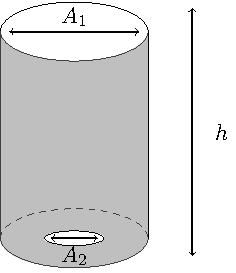
\includegraphics[scale=0.8]{Beker.pdf}    
\end{figure}

%\newpage
%\section{Formules}
%De hoeveelheid volume van een vloeistof dat per tijdseenheid door een zekere oppervlakte passeert, wordt het debiet genoemd. Mathematisch omschreven als volgt:
%\begin{equation}\label{eq:debiet}
 %   Q = \frac{dV}{dt}.
%\end{equation}
%Volume is oppervlakte waardoor het vloeistof maal de hoogte van dit vloeistof. Hieruit volgt dat $Q$ equivalent is aan het volgende:
%\begin{equation}\label{eq:debiet_omschreven}
  %  Q = \frac{dV}{dt} = \frac{dhA}{dt} = A\frac{dh}{dt} = Av.
%\end{equation}
%In \cref{eq:debiet_omschreven} is $v$ de snelheid van vloeistof in \si{\meter\per\second} door oppervlakte $A$.

%Op elke plek in het gevulde gedeelte van het vat is het debiet gelijk. 
%\begin{equation}\label{eq:constant_debiet}
%    Av = \text{constant}
%\end{equation}

%Het doorsnee oppervlakte verschilt weliswaar. Zo is bij het gat $A_1 < A_2$. Uit %\cref{eq:constant_debiet} volgt dan:
%\begin{equation}\label{eq:v_h}
%\begin{split}
 %   A_1\vec{v}_1 = A_2\vec{v}_2\\
  %  \vec{v}_2 = \frac{A_1}{A_2}\vec{v}_1\\
   %  \rightarrow v_2 = -\frac{A_1}{A_2}v_1\\
%    \end{split}
 %   \end{equation}
% Eenheden van een grootheid wordt weergeven als volgt: [grootheid]
%$[v_{\text{stroom}}]$ is gelijk aan \si{\meter\per\second}. Uit \cref{eq:eenheid} volgt dat %$c$ gelijk is aan:
%\begin{equation}\label{eq:eenheid}
%[c] = \frac{[v_{(\text{stroom})}]}{[h]} = \frac{\si{\meter\per\second}}{\si{\meter}} = %\si{\second}^{-1}
%\end{equation}
%De constante $c$ heeft dus als eenheid $\si{\second}^{-1}$

%%%%%%%%%%%%%%%%%%%%%%%%%%%%%%%%%%                         

\newpage
\section{Discussie}
De gestelde hypotheses waren positief. Een wortelverband bestaat tussen $y_f$ en $t$. Verder leverde de grafiek met $v$ uitgezet tegen $t$ een omgekeerde wortelverband. Dit is te verklaren met de wet van Torricelli, namelijk hoogte-energie wordt omgezet in snelheid. De verklaring is weergeven in \cref{eq:wet}.
\begin{equation}\label{eq:wet}
\begin{split}
m \cdot g \cdot y_f = \frac{1}{2} \cdot m \cdot \vec{v^2}\\
\vec{v} = \sqrt{2 \cdot g \cdot y_f}
\end{split}
\end{equation}

\section{Reflectie}
Ik ben tevreden met de resultaten van ons uitgevoerde onderzoek. Daarnaast
ben ik trots op ons verslag. De gegevens zijn op een professionele
manier in het verslag verwerkt met een mooie strakke lay-out. Ik ben minder
tevreden met de meetfouten die zijn gemaakt. Ondanks dat ik de theorie
goed hebben toegepast. Ik heb in deze PO geleerd om onze kennis in
een praktische opdracht toe te passen, waardoor ik de onderzoeksvragen
heb kunnen beantwoorden.


\newpage
\appendix
\section{Logboek}
\begin{table}[ht]
\centering
\caption{Een logboek met de van week van uitvoering, activiteit, tijdspendering.}
\begin{tabular}{Scc}
\toprule
{Week van uitvoering} & Activiteit & Tijdspendering in (\si{\hour})\\
\midrule
6 & Oriënteren & 1\\
7 & Oriënteren & 1\\
8 & Oriënteren & 1\\
9 & Modellering & 2\\
10 & Dataverwerking & 3\\
11 & Dataverwerking & 3\\
12 & Afronding & 2\\
13 & Controle & $\frac{1}{6}$\\
\bottomrule
\end{tabular}
\end{table}
\end{document}
